\documentclass[../../main/main.tex]{subfiles}
\graphicspath{{./figures/}}

\dominitoc
\faketableofcontents

% \renewcommand{\mtcSfont}{\small\bfseries}
% \renewcommand{\mtcSSfont}{\footnotesize}
\mtcsettitle{minitoc}{}
\mtcsetrules{*}{off}

\makeatletter
\renewcommand{\@chapapp}{Chimie -- chapitre}
\makeatother

% \toggletrue{student}
% \toggletrue{corrige}
% \renewcommand{\mycol}{black}
% \renewcommand{\mycol}{gray}

\hfuzz=5.002pt

\begin{document}
\setcounter{chapter}{6}

\settype{book}
\settype{prof}
\settype{stud}

\chapter{Diagrammes potentiel-pH}

% \vspace*{\fill}

\begin{tcb}*(ror)<ctc>{\iconsomm~Sommaire}
	\vspace{-15pt}
	\minitoc
	\vspace{-25pt}
\end{tcb}

% \vspace*{\fill}
% \begin{prgm}
% \small
% \begin{tcb}*(ror)"know"{Savoirs}
% 	\begin{itemize}
% 		\item Principe de construction, lecture et utilisation d'un diagramme
% 		      potentiel-pH.
% 		\item Diagramme potentiel-pH de l'eau.
% 	\end{itemize}
% \end{tcb}
\begin{tcb}*[sidebyside, sidebyside align=top](ror)<ctc>""{\iconhow~Capacités exigibles}
	\small
	\begin{itemize}[label=\rcheck]
		\item Identifier les différents domaines d'un diagramme fourni associés à
		      des espèces chimiques données.
		\item Déterminer la valeur de la pente d'une frontière dans un diagramme
		      potentiel-pH.
		\item Justifier la position d'une frontière verticale.
		\item Déterminer la valeur d'une constante ($\pk$, $\pk[s]$ ou $E^\circ$)
		      à partir d'un diagramme fourni.
	\end{itemize}
	\tcblower
	\begin{itemize}[label=\rcheck]
		\item Prévoir le caractère thermodynamiquement favorisé ou non d'une
		      transformation par superposition de diagrammes.
		\item Prévoir la stabilité des espèces dans l'eau.
		\item Prévoir une dismutation ou médiamutation en fonction du pH du milieu.
		\item Confronter les prévisions à des données expérimentales et
		      interpréter d'éventuels écarts en termes cinétiques.
	\end{itemize}
\end{tcb}
% \end{prgm}
\vspace{-15pt}

% \vspace*{\fill}

% \newpage
%
% \vspace*{\fill}
% {
% \begin{boxes}
\begin{tcb}*[sidebyside](ror)<ctc>{\iconchek~L'essentiel}
	\small
	\begin{tcb}*(defi)<ctc>{\icondefi~Définitions}
		\tcblistof[\paragraph*]{defi}{\hspace*{4.8pt}}
	\end{tcb}
	% \begin{tcb}(rapp)<ctc>{Rappels}
	%   \tcblistof[\paragraph*]{rapp}{\hspace*{4.8pt}}
	% \end{tcb}
	\begin{tcb}*(prop)<ctc>{\iconprop~Propriétés}
		\tcblistof[\paragraph*]{prop}{\hspace*{4.8pt}}
		% \tcblistof[\paragraph*]{loi}{\hspace*{4.8pt}}
		\tcblistof[\paragraph*]{theo}{\hspace*{4.8pt}}
	\end{tcb}
	% \begin{tcb}*(coro)<ctc>{Corollaires}
	%   \tcblistof[\paragraph*]{coro}{\hspace*{4.8pt}}
	% \end{tcb}
	% \begin{tcb}*(demo)<ctc>{Démonstrations}
	%   \tcblistof[\paragraph*]{demo}{\hspace*{4.8pt}}
	%   \tcblistof[\paragraph*]{prev}{\hspace*{4.8pt}}
	% \end{tcb}
	% \begin{tcb}*(inte)<ctc>{Interprétations}
	%   \tcblistof[\paragraph*]{inte}{\hspace*{4.8pt}}
	% \end{tcb}
	\begin{tcb}*(tool)<ctc>{\icontool~Outils}
		\tcblistof[\paragraph*]{tool}{\hspace*{4.8pt}}
	\end{tcb}
	% \begin{tcb}*(nota)<ctc>{Notations}
	%   \tcblistof[\paragraph*]{nota}{\hspace*{4.8pt}}
	% \end{tcb}
	% \begin{tcb}*(appl)<ctc>{Applications}
	%   \tcblistof[\paragraph*]{appl}{\hspace*{4.8pt}}
	% \end{tcb}
	% \begin{tcb}*(rema)<ctc>{Remarques}
	%   \tcblistof[\paragraph*]{rema}{\hspace*{4.8pt}}
	% \end{tcb}
	% \begin{tcb}*(exem)<ctc>{Exemples}
	%   \tcblistof[\paragraph*]{exem}{\hspace*{4.8pt}}
	% \end{tcb}
	% \begin{tcb}*(ror)<ctc>{Points importants}
	%   \tcblistof[\paragraph*]{ror}{\hspace*{4.8pt}}
	% \end{tcb}
	% \begin{tcb}*(impo)<ctc>{Erreurs communes}
	%   \tcblistof[\paragraph*]{impo}{\hspace*{4.8pt}}
	% \end{tcb}
	\tcblower
	\small
	% \begin{tcb}*(defi)<ctc>{Définitions}
	%   \tcblistof[\paragraph*]{defi}{\hspace*{4.8pt}}
	% \end{tcb}
	% \begin{tcb}*(rapp)<ctc>{Rappels}
	%   \tcblistof[\paragraph*]{rapp}{\hspace*{4.8pt}}
	% \end{tcb}
	% \begin{tcb}*(prop)<ctc>{Propriétés}
	%   \tcblistof[\paragraph*]{prop}{\hspace*{4.8pt}}
	% > \tcblistof[\paragraph*]{loi}{\hspace*{4.8pt}}
	%   \tcblistof[\paragraph*]{theo}{\hspace*{4.8pt}}
	% \end{tcb}
	% \begin{tcb}*(coro)<ctc>{Corollaires}
	%   \tcblistof[\paragraph*]{coro}{\hspace*{4.8pt}}
	% \end{tcb}
	% \begin{tcb}*(demo)<ctc>{Démonstrations}
	%   \tcblistof[\paragraph*]{demo}{\hspace*{4.8pt}}
	%   \tcblistof[\paragraph*]{prev}{\hspace*{4.8pt}}
	% \end{tcb}
	% \begin{tcb}*(inte)<ctc>{Interprétations}
	%   \tcblistof[\paragraph*]{inte}{\hspace*{4.8pt}}
	% \end{tcb}
	% \begin{tcb}*(tool)<ctc>{Outils}
	%   \tcblistof[\paragraph*]{tool}{\hspace*{4.8pt}}
	% \end{tcb}
	% \begin{tcb}*(nota)<ctc>{Notations}
	%   \tcblistof[\paragraph*]{nota}{\hspace*{4.8pt}}
	% \end{tcb}
	\begin{tcb}*(appl)<ctc>{\iconappl~Applications}
		\tcblistof[\paragraph*]{appl}{\hspace*{4.8pt}}
	\end{tcb}
	% \begin{tcb}*(rema)<ctc>{Remarques}
	%   \tcblistof[\paragraph*]{rema}{\hspace*{4.8pt}}
	% \end{tcb}
	% \begin{tcb}*(exem)<ctc>{Exemples}
	%   \tcblistof[\paragraph*]{exem}{\hspace*{4.8pt}}
	% \end{tcb}
	\begin{tcb}*(ror)<ctc>{\iconhart~Points importants}
		\tcblistof[\paragraph*]{ror}{\hspace*{4.8pt}}
	\end{tcb}
	\begin{tcb}*(impo)<ctc>{\iconimpo~Erreurs communes}
		\tcblistof[\paragraph*]{impo}{\hspace*{4.8pt}}
	\end{tcb}
\end{tcb}

% \end{boxes}
% }
% \vspace*{\fill}
\newpage

\section{Présentation}
\subsection{Nécessité des diagrammes $E-\pH$}
Nous avons vu dans les chapitres précédents que les couples acido-basiques
possédaient des domaines de prédominance (ou d'existence) en fonction du pH, et
que les couples d'oxydoréduction possédaient des domaines de prédominance en
fonction du potentiel. Ainsi, les couples rédox présentant des comportement
acido-basiques possèdent des diagrammes de prédominance en fonction de ces deux
paramètres.

\begin{tcb*}(defi){Diagramme potentiel-pH}
	Une espèce chimique conjuguée à d'autres espèces \textit{via} plusieurs
	couples acido-basiques et rédox possède des domaines représentables en
	fonction du \textbf{potentiel} (en ordonnée) et du \textbf{pH} (en abscisse).
\end{tcb*}

\begin{tcb*}(exem)<lftt>{Diagramme $E-\pH$ de l'aluminium}
	\begin{center}
		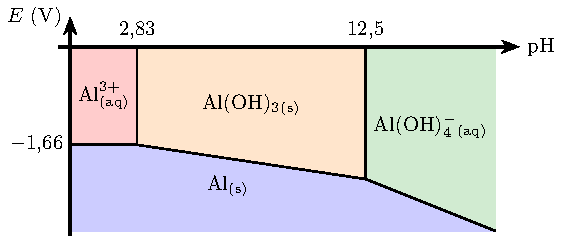
\includegraphics[scale=1.5]{eph_al}
		\captionof{figure}{Diagramme $E-\pH$ de l'aluminium.}
	\end{center}
	On note que l'on a bien besoin de la donnée combinée du pH \textbf{et} du
	potentiel pour déterminer quelle forme domine.
\end{tcb*}

\subsection{Analyse d'un diagramme $E-\pH$}
\begin{tcb*}[breakable](ror){Frontières d'un diagramme $E-\pH$}
	On distingue trois types de frontières sur l'exemple précédent~:
	\begin{itemize}
		\bitem{Frontière horizontale}~: sépare un \xul{\psw{\textbf{couple purement
					rédox}}}, donc \xul{\psw{\textbf{de \no différents}}}.
		% Le nombre d'oxydation \xul{\psw{\textbf{augmente de bas en haut}}}.
		\bitem{Frontière verticale}~: sépare un \xul{\psw{\textbf{couple purement
					acide-base}}}, donc \xul{\psw{de même n.o}}.
		% Les espèces acides sont \xul{\psw{à gauche}}, les espèces basiques
		% \xul{\psw{à droite}}.
		\bitem{Frontière inclinée}~: sépare un couple \xul{\psw{\textbf{à la fois
					rédox et AB}}}.
	\end{itemize}
	Ainsi, on trouvera qualitativement les espèces en fonction du pH et du
	potentiel telles que~:
	\begin{itemize}
		\bitem{Bas pH} = \xul{\psw{acide}}~; \textbf{haut pH} = \xul{\psw{base}}.
		\bitem{Bas $E$} = \xul{\psw{réducteur}}~; \textbf{haut $E$} =
		\xul{\psw{oxydant}}.
	\end{itemize}
\end{tcb*}

\subsection{Diagramme $E-\pH$ de l'eau}
La connaissance du diagramme de l'eau s'avèrera primordiale pour l'étude des
réactions aqueuses (voir~\fullref{--}{sec:util}).

\begin{tcb*}(defi){Couples rédox de l'eau}
	L'eau $\ce{H_2O_{\rm(l)}}$ intervient dans deux couples rédox~:
	\begin{tasks}[label=$\scaleto{\diamond}{7pt}$](2)
		\task \psw{$\ce{O2_{\rm(g)}/H_2O_{\rm(l)}}$~;}
		\task \psw{$\ce{H_2O_{\rm(l)}/H_2{\rm(g)}}$.}
	\end{tasks}
\end{tcb*}

\begin{tcb*}[breakable](appl)<lftt>{Tracé du diagramme de l'eau}
	Tracer le diagramme $E-\pH$ de l'eau. On prendra comme convention de tracé
	$p_t = p^\circ$. On donne $E^\circ(\ce{O2_{\rm(g)}/H_2O_{\rm(l)}}) = E_1^\circ
		= \SI{1.23}{V}$ et $E^\circ(\ce{H_2O_{\rm(l)}/H_2{\rm(g)}}) = \SI{0.00}{V}$.
	\tcblower
	On écrit les demi-équations associées puis les potentiels~:
	\begin{itemize}
		\item $\ce{O2_{\rm(g)}/H_2O_{\rm(l)}}$~:
		      \vspace{-20pt}
		      \begin{gather*}
			      \ce{
			      \psw{2 {H_2O}_{\rm(l)}}
			      =
			      \psw{{O_2}_{\rm(g)} + 4 {H}^+_{\rm(aq)} +4 e^-}
			      }
			      \\\Ra
			      E_1 =
			      \psw{
				      E_1^\circ + \frac{\num{0.06}}{4} \log (\frac{[\ce{H+}]^4
					      p_{\ce{O_2}}}{{c^\circ}^4 p^\circ})
			      }
			      \\\Lra
			      E_1 =
			      \psw{
				      E_1^\circ - \num{0.06}\pH + \num{0.06}\log (\frac{p_{\ce{O_2}}}{p^\circ})
			      }
			      \\\shortintertext{
				      Or, $\ce{{O_2}_{\rm(g)}}$ prédomine
				      $\Lra \DS
					      \psw{
						      p_{\ce{O_2}} > p_t = p^\circ
						      \Ra
						      \log (\frac{p_{\ce{O_2}}}{p^\circ}) >
						      \log (\frac{p_t}{p^\circ}) = 0
					      }
				      $
			      }
			      \beforetext{d'où}
			      \psw{E_1 > E_1^\circ - \num{0.06}\pH}
			      \Lra
			      \setlength{\fboxsep}{3mm}
			      \boxed{\psw{E\ind{front} = \num{1.23} - \num{0.06}\pH}}
		      \end{gather*}
		\item $\ce{H_2O_{\rm(l)}/H_2{\rm(g)}}$~:
		      \vspace{-20pt}
		      \begin{gather*}
			      \ce{
			      \psw{{H_2}_{\rm(g)}}
			      =
			      \psw{2H^+_{\rm(aq)} + 2e^-}
			      }
			      \\\Ra
			      E_2 =
			      \psw{
				      E_2^\circ + \frac{\num{0.06}}{2} \log (\frac{[\ce{H^+}]^2
					      p^\circ}{{c^\circ}^2 p_{\ce{H_2}}})
			      }
			      \\\Lra
			      E_2 =
			      \psw{
				      E_2^\circ - \num{0.06}\pH + \num{0.06}\log (\frac{p^\circ}{p_{\ce{H_2}}})
			      }
			      \\\shortintertext{
				      Or, $\ce{{H_2}_{\rm(g)}}$ prédomine
				      $\Lra \DS
					      \psw{
						      p_{\ce{H_2}} > p_t = p^\circ
						      \Ra
						      \log (\frac{p^\circ}{p_{\ce{H_2}}}) <
						      \log (\frac{p^\circ}{p_t}) = 1
					      }
				      $
			      }
			      \beforetext{d'où}
			      \psw{E_2 < \num{-0.06}\pH}
			      \Lra
			      \setlength{\fboxsep}{3mm}
			      \boxed{\psw{E\ind{front} = -\num{0.06}\pH}}
		      \end{gather*}
	\end{itemize}
	\vspace{-10pt}
	\begin{center}
		\sswitch{
			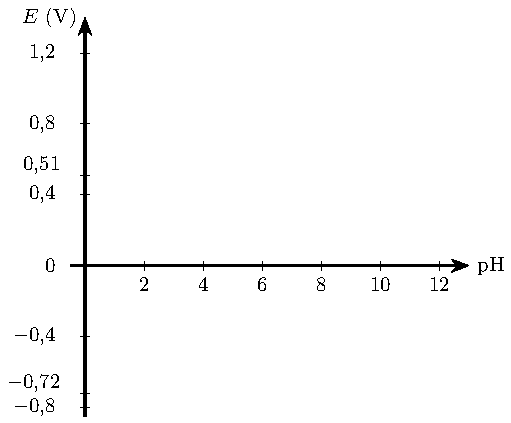
\includegraphics[width=.5\linewidth]{eph_eau-plain}
		}{
			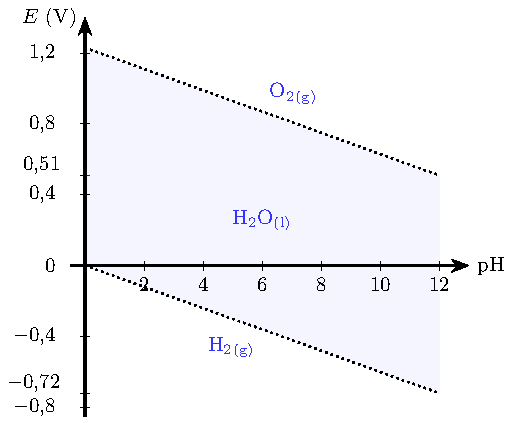
\includegraphics[width=.5\linewidth]{eph_eau}
		}
		\vspace{-10pt}
		\captionof{figure}{Diagramme $E-\pH$ de l'eau.}
	\end{center}
\end{tcb*}

\section{Construction et lecture}

La plupart du temps, on dispose de l'allure du diagramme $E-\pH$ d'une espèce,
mais ses différentes formes ne sont pas indiquées sur le diagramme, elles sont
données à part. Il est alors question d'identifier quelle zone du diagramme
correspond à quelle espèce, puis de déterminer la position ou les équations des
frontières.

\subsection{Remplissage des espèces}

\begin{tcb*}(tool){Placer les espèces d'un diagramme}
	\begin{enumerate}[label=\sqenumi]
		\item Déterminer les \textbf{\no de l'élément} dans chacune des espèces
		      données~;
		\item Déterminer le caractère \textbf{acide ou basique} de chaque espèce de
		      \textbf{même \no}~;
		\item Tracer un diagramme simplifié sans frontière inclinée, aussi appelé
		      \textbf{diagramme de situation}~:
		      \begin{itemize}[label=$\scaleto{\triangleright}{7pt}$]
			      \item Le nombre d'oxydation \xul{\psw{\textbf{augmente de bas en haut}}}.
			      \item Les espèces acides sont \xul{\psw{à gauche}}, les espèces basiques
			            \xul{\psw{à droite}}.
		      \end{itemize}
	\end{enumerate}
\end{tcb*}

\begin{tcb*}[breakable](appl)<lftt>{Placement des espèces du fer}
	\noindent
	\begin{minipage}[c]{.5\linewidth}
		On donne l'allure du diagramme du fer ci-contre. Les espèces à placer sont
		$\ce{Fe}_{\rm(s)}$, $\ce{{Fe}^2+_{\rm(aq)}}$, $\ce{{Fe}^3+_{\rm(aq)}}$,
		$\ce{{Fe(OH)_2}_{\rm(s)}}$ et $\ce{{Fe(OH)_3}_{\rm(s)}}$.
	\end{minipage}
	\begin{minipage}[c]{.5\linewidth}
		\vspace{0pt}
		\begin{center}
			\sswitch{
				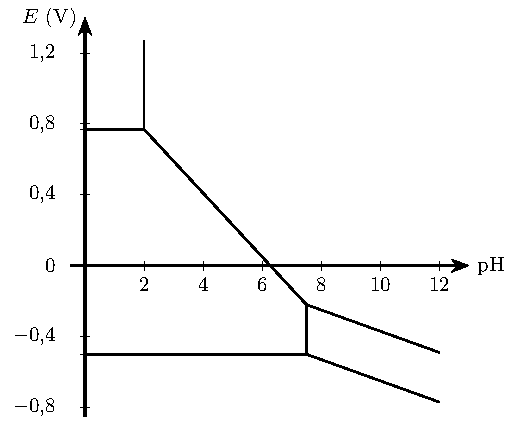
\includegraphics[width=\linewidth]{eph_fer-plain}
			}{
				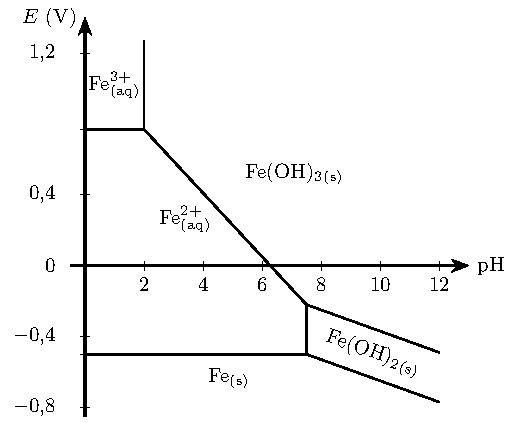
\includegraphics[width=\linewidth]{eph_fer-filled}
			}
		\end{center}
	\end{minipage}
	\tcblower
	\begin{enumerate}[label=\sqenumi]
		\bitem{Nombres d'oxydation}~:
		\begin{center}
			\begin{tabularx}{.6\linewidth}{YYYYY}
				\toprule
				$\ce{Fe}_{\rm(s)}$         &
				$\ce{{Fe}^2+_{\rm(aq)}}$   &
				$\ce{{Fe}^3+_{\rm(aq)}}$   &
				$\ce{{Fe(OH)_2}_{\rm(s)}}$ &
				$\ce{{Fe(OH)_3}_{\rm(s)}}$
				\\\addlinespace[.5em]
				\psw{0}                    &
				\psw{+\myRoman{2}}         &
				\psw{+\myRoman{3}}         &
				\psw{+\myRoman{2}}         &
				\psw{+\myRoman{3}}
				\\
				\bottomrule
			\end{tabularx}
		\end{center}
		\bitem{Espèces basiques}~:
		\begin{align*}
			\beforetext{$\no{Fe} = +\myRoman{2}$~:}
			\ce{
			\psw{{Fe}^{2+}_{\rm(aq)} + 2 {HO}^-_{\rm(aq)}}
			 & =
			\psw{{Fe(OH)_2}_{\rm(s)}}
			}
			\tag*{}
			\\\beforetext{\hspace{2.5cm}$\Lra$}
			\ce{
			\psw{{Fe}^{2+}_{\rm(aq)} + 2 {H_2O}_{\rm(l)}}
			 & =
			\psw{{Fe(OH)_2}_{\rm(s)} + 2 {H}^+_{\rm(aq)}}
			}
			\tag*{$\mathllap{\text{couple \psw{\ce{Fe^2+}}/\psw{\ce{Fe(OH)_2}}}}$}
			\\\beforetext{$\no{Fe} = +\myRoman{3}$~:}
			\ce{
			\psw{{Fe}^{3+}_{\rm(aq)} + 3 {HO}^-_{\rm(aq)}}
			 & =
			\psw{{Fe(OH)_3}_{\rm(s)}}
			}
			\\\beforetext{\hspace{2.5cm}$\Lra$}
			\ce{
			\psw{{Fe}^{3+}_{\rm(aq)} + 3 {H_2O}_{\rm(l)}}
			 & =
			\psw{{Fe(OH)_3}_{\rm(s)} + 3 {H}^+_{\rm(aq)}}
			}
			\tag*{$\mathllap{\text{couple \psw{\ce{Fe^3+}}/\psw{\ce{Fe(OH)_3}}}}$}
		\end{align*}
		\bitem{Diagramme de situation}~:
		\begin{center}
			\sswitch{
				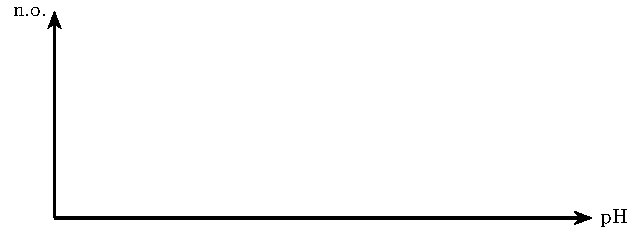
\includegraphics[width=.8\linewidth]{esit_fer-plain}
			}{
				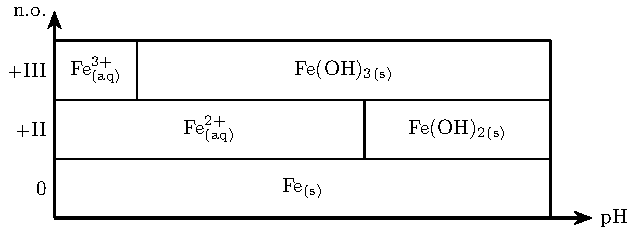
\includegraphics[width=.8\linewidth]{esit_fer}
			}
		\end{center}
	\end{enumerate}
\end{tcb*}

\begin{tcb*}(rema)<lftt>{Caractère acido-basique des solides hydroxydes}
	Écrire les réactions acide-base permet de se convaincre définitivement de qui
	est l'acide et qui est la base, mais en réalité il est évident qu'un composé
	susceptible de \textbf{céder un ion \ce{HO^-}} est une \textbf{espèce
		basique}~; grâce à l'autoprotolyse de l'eau, la définition du chapitre 4
	s'inverse entre donneur et receveur quand on change le composé de transfert
	(\ce{H^+} ou \ce{HO^-}).
\end{tcb*}

\subsection{Position des frontières}
Une fois les espèces placées, on cherche les valeurs remarquables d'un
diagramme~: \textbf{position} d'une frontière verticale ou horizontale ou
\textbf{pente} d'une frontière inclinée.

\begin{tcb*}(tool){Placer les frontières d'un diagramme}
	\begin{enumerate}[label=\sqenumi]
		\bitem{Frontières horizontales}~: comme elles séparent des couples rédox, on
		trouve la limite comme pour les diagrammes de prédominance rédox~:
		\[
			\setlength{\fboxsep}{3mm}
			\boxed{\psw{E\ind{front} = E\ind{lim}}}
			\qav
			\psw{
				\left\{
				\begin{array}{ll}
					[\ce{X}_{\rm(aq)}]\ind{front} & = c_t
					\\
					p_{\ce{X}_{\rm(g)},\rm front} & = p_t
				\end{array}
				\right.
			}
			\quad \text{convention de tracé à la frontière}
		\]
		\bitem{Frontières verticales}~: comme elles séparent des couples acide-base
		de même nombre d'oxydation, on trouve les limites des diagrammes de
		prédominance ou d'existence~:
		\begin{itemize}
			\item Si espèces dissoutes,
			      $\setlength{\fboxsep}{3mm}\boxed{\psw{\pH\ind{front} = \pk}}$~;
			\item Si précipité, \xul{\psw{$\pH\ind{front}$ dépend de $\pk[s]$ et de
					      $c_t|p_t$}}.
		\end{itemize}
		\bitem{Frontières inclinées}~: on exprime $E(\ce{Ox/Red})$ en fonction du
		$\pH$ pour trouver la pente.
	\end{enumerate}
\end{tcb*}

\begin{tcb*}[breakable](appl)<lftt>{Placement des frontières du fer}
	\noindent
	\begin{minipage}[c]{.67\linewidth}
		On rappelle ci-contre le diagramme du fer. On donne de plus
		\begin{itemize}
			\item $E_1^\circ(\ce{{Fe}^2+_{\rm(aq)}/Fe}) = \SI{-.44}{V}$~;
			      $E_2^\circ(\ce{{Fe}^3+_{\rm(aq)}/{Fe}^2+_{\rm(aq)}}) = \SI{0.77}{V}$~;
			\item $\pk[s,2] = \pk[s](\ce{Fe(OH)_2}) = 15$ et $\pk[s,3] =
				      \pk[s](\ce{Fe(OH)_3}) = 38$~;
			\item Convention de tracé $c_t = \SI{0.01}{mol.L^{-1}}$.
		\end{itemize}
		\textbf{Déterminer la position des frontières horizontales et verticales,
			puis les pentes des frontières inclinées}.
	\end{minipage}
	% \hfill
	\begin{minipage}[c]{.30\linewidth}
		\vspace{0pt}
		\begin{center}
			\sswitch{
				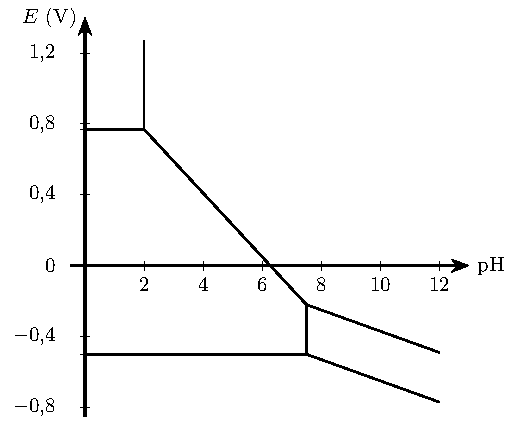
\includegraphics[width=1.1\linewidth]{eph_fer-plain}
			}{
				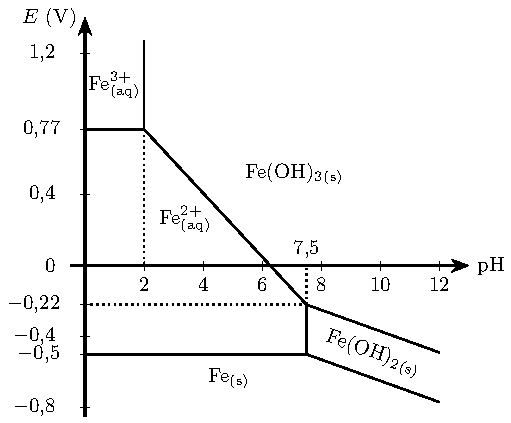
\includegraphics[width=1.1\linewidth]{eph_fer}
			}
		\end{center}
	\end{minipage}
	\tcblower
	\begin{enumerate}[label=\sqenumi]
		\bitem{Frontières horizontales}~: ce sont celles des couples
		$\ce{{Fe}^2+_{\rm(aq)}/Fe}$ et $\ce{{Fe}^3+_{\rm(aq)}/{Fe}^2+_{\rm(aq)}}$.
		\begin{itemize}
			\item
			      \leftcenters{%
			      $\ce{{Fe}^2+_{\rm(aq)}}/\ce{Fe_{\rm(s)}}$~:
			      }{%
			      \psw{$\ce{Fe_{\rm(s)} = {Fe}^2+_{\rm(aq)} + 2e^-}$}
			      }
			      \vspace{-15pt}
			      \begin{align*}
				      \beforetext{\hspace{2.5cm}$\Ra$}
				      E_1
				                     & =
				      \psw{%
					      E_1^\circ \left( \ce{Fe^2+}/\ce{Fe} \right) +
					      \frac{\num{0.06}}{2} \log \frac{[\ce{Fe^2+}]}{c^\circ}
				      }%
				      \\
				      \beforetext{$[\ce{X}_{\rm(aq)}]\ind{front} = c_t \Ra $}
				      E\ind{1,front} & =
				      \psw{E_1^\circ + \frac{\num{0.06}}{2}\log \frac{c_t}{c^\circ}}
				      \\
				      \beforetext{$c_t = \SI{e-2}{mol.L^{-1}} \Ra$}
				      \makebox[0pt][l]{$\xul{\phantom{E\ind{1,front} = - \SI{0.5}{V}}}$}
				      E\ind{1,front} & =
				      \psw{- \SI{0.5}{V}}
			      \end{align*}
			      \vspace{-15pt}
			\item
			      \leftcenters{%
			      $\ce{{Fe}^3+_{\rm(aq)}}/\ce{{Fe}^2+_{\rm(aq)}}$~:
			      }{%
			      \psw{$\ce{{Fe}^2+_{\rm(aq)} = {Fe}^3+_{\rm(aq)} + e^-}$}
			      }
			      \vspace{-15pt}
			      \psw{%
				      \begin{align*}
					      \beforetext{\hspace{2.5cm}$\Ra$}
					      E_2            & = E_2^\circ \left( \ce{Fe^3+}/\ce{Fe^2+} \right) +
					      \num{0.06} \log \frac{[\ce{Fe^2+}]}{[\ce{Fe^2+}]}
					      \\
					      \beforetext{$[\ce{X}_{\rm(g)}]\ind{front} = c_t \Ra $}
					      \makebox[0pt][l]{$\xul{\phantom{E\ind{2,front} = E_2^\circ = \SI{0.77}{V}}}$}
					      E\ind{2,front} & =
					      E_2^\circ = \SI{0.77}{V}
				      \end{align*}
			      }%
		\end{itemize}
		\vspace{-15pt}
		\bitem{Frontières verticales}~:
		Ce sont les frontières des couples acide-base déterminés plus tôt~:
		\begin{itemize}
			\item
			      \leftcentersright{%
			      $\ce{{Fe}^2+_{\rm(aq)}/{Fe(OH)_2}_{\rm(s)}}$~:
			      }{%
			      \psw{$\ce{{Fe(OH)_2}_{\rm(s)} = {Fe}^2+_{\rm(aq)} + 2 {HO}^-_{\rm(aq)}}$}
			      }{%
			      $K_{s,2}$
			      }%
			      \vspace{-15pt}
			      \begin{align*}
				      \beforetext{Condition précipité~:}
				      K_{s,2}
				                     & =
				      \psw{\frac{[\ce{HO^-}]^2\ind{front}[\ce{Fe^2+}]\ind{front}}{{c^\circ}^3}}
				      \\\Lra
				      \pk[s,2]       & =
				      \psw{2\pOH\ind{front} - \log c_t/c^\circ}
				      \\\Lra
				      \beforetext{$\pOH = \pk[e] - \pH$~:}
				      \Aboxed{
					      \pH\ind{front}
				                     & =
					      \psw{\pk[e] - \frac{1}{2}\pk[s,2] - \frac{1}{2} \log c_t/c^\circ}
				      }
				      \\\Lra
				      \makebox[0pt][l]{$\xul{\phantom{\xul{\pH\ind{front} = \num{7.5}}}}$}
				      \pH\ind{front} & =
				      \psw{\num{7.5}}
			      \end{align*}
			\item
			      \leftcentersright{%
			      $\ce{{Fe}^3+_{\rm(aq)}/{Fe(OH)_3}_{\rm(s)}}$~:
			      }{%
			      \psw{$\ce{{Fe(OH)_3}_{\rm(s)} = {Fe}^3+_{\rm(aq)} + 3 {HO}^-_{\rm(aq)}}$}
			      }{%
			      $K_{s,3}$
			      }%
			      \vspace{-15pt}
			      \psw{%
				      \begin{align*}
					      \beforetext{Condition précipité~:}
					      K_{s,3}
					                     & =
					      \frac{[\ce{HO^-}]^3\ind{front}[\ce{Fe^3+}]\ind{front}}{{c^\circ}^4}
					      \\\Lra
					      \pk[s,3]       & = 3\pOH\ind{front} - \log c_t/c^\circ
					      \\\Lra
					      \beforetext{$\pOH = \pk[e] - \pH$~:}
					      \Aboxed{
						      \pH\ind{front}
					                     & =
						      \pk[e] - \frac{1}{3}\pk[s,3] - \frac{1}{3} \log c_t/c^\circ
					      }
					      \\\Lra
					      \makebox[0pt][l]{$\xul{\phantom{\xul{\pH\ind{front} = \num{2.0}}}}$}
					      \pH\ind{front} & = \num{2.0}
				      \end{align*}
			      }%
		\end{itemize}
		\vspace{-15pt}
		\bitem{Frontières inclinées}~: on étudie la \textbf{pente} des équilibres
		restants~:
		\begin{itemize}
			\item
			      \leftcenters{%
			      $\ce{{Fe(OH)_2}_{\rm(s)}/Fe_{\rm(s)}}$~:
			      }{%
			      $\psw{\ce{
				      Fe_{\rm(s)} + 2 H_2O_{\rm(l)}
					      =
					      {Fe(OH)_2}_{\rm(s)} + 2 {H}^+_{\rm(aq)} + 2e^-
				      }}$
			      }%
			      \vspace{-15pt}
			      \psw{%
				      \begin{align*}
					      E\ind{front} & =
					      E^\circ(\ce{{Fe(OH)_2}_{\rm(s)}/Fe_{\rm(s)}}) + \frac{\num{0.06}}{2}
					      \log [\ce{H^+}]^2
					      \\\Lra
					      E\ind{front} & =
					      E^\circ(\ce{{Fe(OH)_2}_{\rm(s)}/Fe_{\rm(s)}}) - \xul{\num{0.06}\pH}
				      \end{align*}
			      }%
			      \vspace{-15pt}
			\item
			      \leftcenters{%
			      $\ce{{Fe(OH)_3}_{\rm(s)}/{Fe}^2+_{\rm(aq)}}$~:
			      }{%
			      $\psw{\ce{
				      {Fe}^2+_{\rm(aq)} + 3 H_2O_{\rm(l)}
					      =
					      {Fe(OH)_3}_{\rm(s)} + 3 {H}^+_{\rm(aq)} + 3e^-
				      }}$
			      }%
			      \vspace{-15pt}
			      \psw{%
				      \begin{align*}
					      E\ind{front} & =
					      E^\circ(\ce{{Fe(OH)_3}_{\rm(s)}/{Fe}^2+_{\rm(aq)}}) + \num{0.06}
					      \log \frac{[\ce{H^+}]^3}{c_t}
					      \\\Lra
					      E\ind{front} & =
					      E^\circ(\ce{{Fe(OH)_3}_{\rm(s)}/{Fe}^2+_{\rm(aq)}}) -
					      \xul{\num{0.18}\pH} -
					      \num{0.06} \log c_t
				      \end{align*}
			      }%
			      \vspace{-15pt}
			\item
			      \leftcenters{%
			      $\ce{{Fe(OH)_3}_{\rm(s)}/{Fe(OH)_2}_{\rm(s)}}$~:
			      }{%
			      \hspace{20pt}
			      $\psw{\ce{
				      {Fe(OH)_2}_{\rm(s)} + H_2O_{\rm(l)}
					      =
					      {Fe(OH)_3}_{\rm(s)} + {H}^+_{\rm(aq)} + e^-
				      }}$
			      }%
			      \vspace{-15pt}
			      \psw{%
				      \begin{align*}
					      E\ind{front} & =
					      E^\circ(\ce{{Fe(OH)_3}_{\rm(s)}/{Fe(OH)_2}_{\rm(s)}}) + \num{0.06}
					      \log [\ce{H^+}]
					      \\\Lra
					      E\ind{front} & =
					      E^\circ(\ce{{Fe(OH)_3}_{\rm(s)}/{Fe(OH)_2}_{\rm(s)}}) - \xul{\num{0.06}\pH}
				      \end{align*}
			      }%
			      \vspace{-15pt}
		\end{itemize}
	\end{enumerate}
	\begin{center}
		\sswitch{
			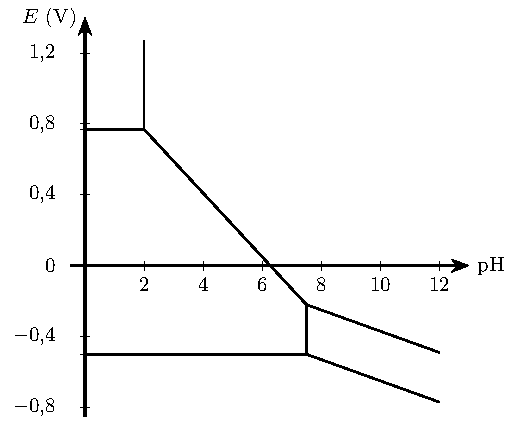
\includegraphics[width=.6\linewidth]{eph_fer-plain}
		}{
			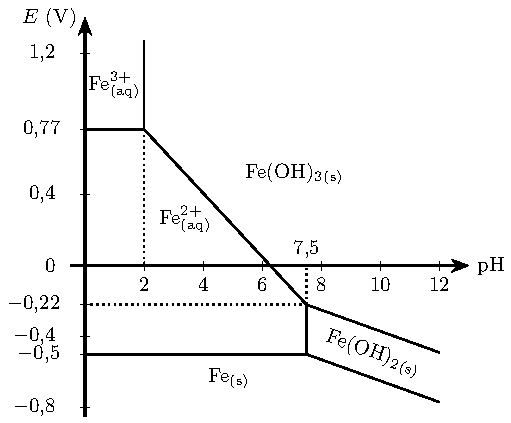
\includegraphics[width=.6\linewidth]{eph_fer}
		}
		\captionof{figure}{Diagramme $E-\pH$ du fer complété.}
	\end{center}
\end{tcb*}

\section{Utilisation des diagrammes $E-\pH$}
\label{sec:util}

\subsection{Sens spontané de réaction}
\begin{tcb*}[sidebyside, righthand ratio=.4](ror){Sens spontané de réaction}
	Comme dans le chapitre précédent, \textbf{l'oxydant le plus fort} réagit avec
	\textbf{le réducteur le plus fort}~; cependant, la force ne dépend plus
	uniquement de $E^\circ$ mais \textbf{dépend du potentiel total} $E$.
	\smallbreak
	On le repère sur un diagramme $E-\pH$ en regardant \textbf{quelles espèces ont
		des domaines disjoints}.
	\tcblower
	\begin{center}
		\sswitch{
			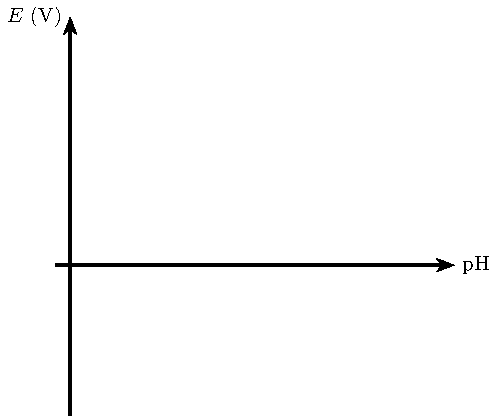
\includegraphics[width=\linewidth]{eph_gen-plain}
		}{
			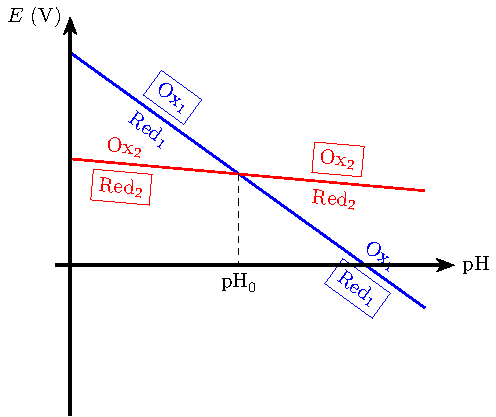
\includegraphics[width=\linewidth]{eph_gen}
		}
		\vspace{-15pt}
		\captionof{figure}{Sens spontané $E-\pH$}
	\end{center}
\end{tcb*}

\subsection{Stabilité d'une espèce dans l'eau}
Le plus souvent, on s'intéresse au sens spontané de réaction d'une
\textbf{espèce en contact avec l'eau}, par exemple pour conclure quant à la
possibilité de rouille. On utilise pour ça la \textbf{superposition des
	diagrammes}~:
\begin{tcbraster}[raster equal height=rows, raster columns=2]
	\begin{tcb*}(prop){Stabilité dans l'eau}
		À pH fixé, s'il existe un domaine de \textbf{potentiel commun} entre
		\textbf{l'eau et l'espèce étudiée} en superposant leurs diagrammes, alors
		l'espèce en question est \textbf{stable dans l'eau}.
		\bigbreak
		Dans le cas du fer, seul le $\ce{Fe_{\rm(s)}}$ n'est pas stable dans l'eau,
		et pourra d'une part se transformer en $\ce{{Fe}^2+_{\rm(aq)}}$ puis
		ultimement de $\ce{{Fe(OH)_2}_{\rm(s)}}$~: c'est de la rouille~!
	\end{tcb*}
	\begin{tcb*}(exem)<rgtt>'r'{Stabilité du fer dans l'eau}
		\begin{center}
			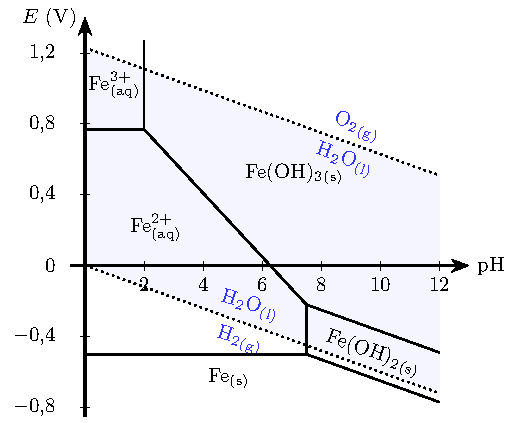
\includegraphics[width=\linewidth]{eph_fer-eau}
			\captionof{figure}{Stabilité du fer dans l'eau}
		\end{center}
	\end{tcb*}
\end{tcbraster}

\begin{tcb*}(impo){Stabilité et cinétique}
	Tous les chapitres étudiés ne portent que sur les \textbf{équilibres}
	chimiques. Mis à part le chapitre traitant spécifiquement de cinétique, toutes
	nos conclusions de sont que pour $t \to \infty$~!
	\smallbreak
	Ainsi, une espèce peut très bien être instable dans l'eau et avoir une
	réaction totale avec elle tout en n'étant que \textbf{très lentement rongée}
	par elle. C'est notamment ce qu'on étudie dans la science de la corrosion.
\end{tcb*}

\subsection{Cas particuliers des dismutations}
% On a vu des réactions rédox particulières au chapitre précédent~: les
% \textbf{dismutations} et les \textbf{médiamutations}. Nous les avions étudiées
% en fonction d'un simple échelle en $E^\circ$~; voyons ce qu'elles donnent en
% diagrammes $E-\pH$ sur un exemple.

\begin{tcb*}[sidebyside, sidebyside align=top](exem)<lftt>{Dismutation/médiamutation de l'iode}
	Sans prendre en compte les réactions de dismutation et de médiamutation, le
	diagramme de l'iode a l'allure suivante~:
	\begin{center}
		\sswitch{
			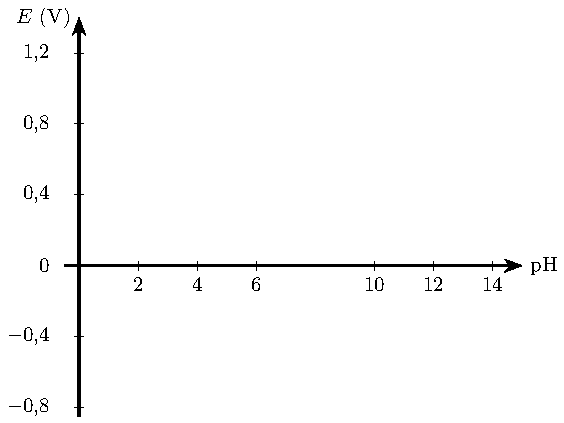
\includegraphics[width=\linewidth]{eph_iode-plain}
		}{
			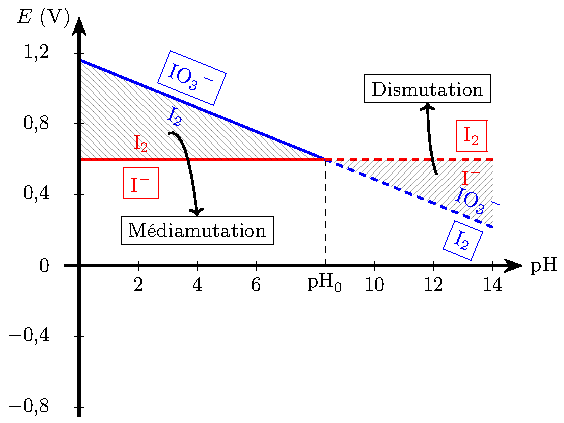
\includegraphics[width=\linewidth]{eph_iode-avant}
		}
		\vspace{-15pt}
		\captionof{figure}{Iode sans dismutation.}
	\end{center}
	% On remarque ainsi qu'à partir de $\pH \gtrsim 8$, le diiode réagit sur
	% lui-même pour former $\ce{I-}$ et $\ce{IO_3^-}$.
	\tcblower
	Pour $\pH \gtrsim 8$, le diiode réagit sur lui-même pour former $\ce{I-}$ et
	$\ce{IO_3^-}$~; il reste le couple \ce{IO3^-/I-}~:
	% Il faut ainsi étudier le couple \ce{IO3^-/I-} pour tracer la seconde partie du
	% diagramme. On obtient alors~:
	\begin{center}
		\sswitch{
			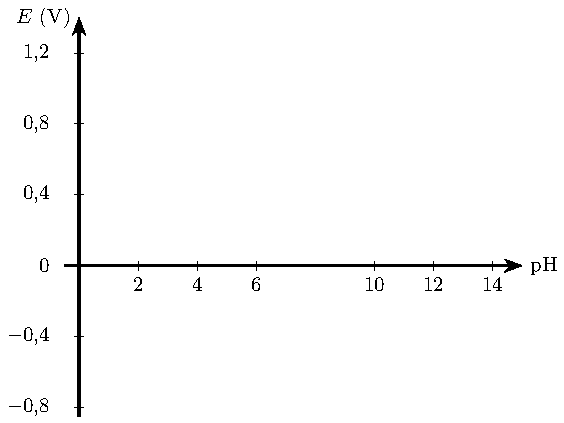
\includegraphics[width=\linewidth]{eph_iode-plain}
		}{
			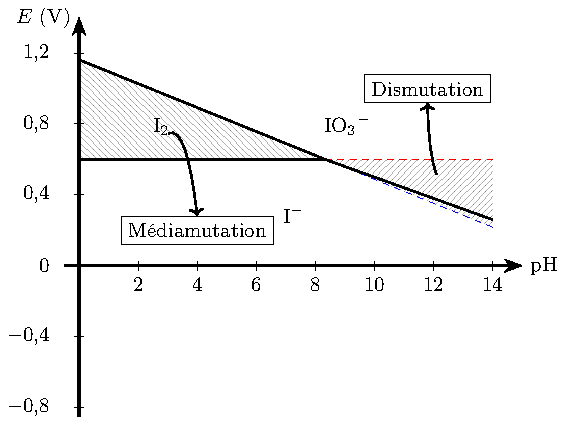
\includegraphics[width=\linewidth]{eph_iode-apres}
		}
		\vspace{-15pt}
		\captionof{figure}{Iode avec dismutation.}
	\end{center}
	% Ainsi, les réactions de dismutation et de médiamutation sont facilement
	% remarques sur des diagrammes $E-\pH$.
\end{tcb*}

\begin{tcb*}(inte)<lftt>{Repérer une dismutation sur un diagramme}
	% Ainsi, on peut en conclure~:
	\begin{itemize}
		\item \textbf{Disparition d'une frontière} $\Lra$ \xul{\psw{dismutation}}~;
		\item \textbf{Domaine en triangle} $\Lra$ \xul{\psw{médiamutation}}.
	\end{itemize}
\end{tcb*}
\vspace{-15pt}

\end{document}
